\begin{figure}[htbp]
\centering
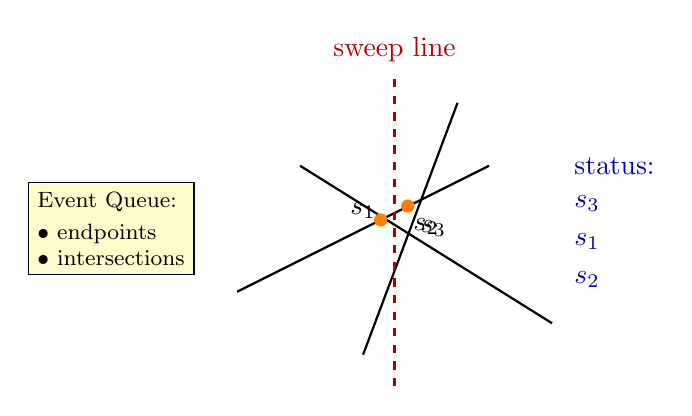
\begin{tikzpicture}[scale=0.8]
  \draw[thick] (0,1)--(4,3) node[midway,above] {$s_1$};
  \draw[thick] (1,3)--(5,0.5) node[midway,above] {$s_2$};
  \draw[thick] (2,0)--(3.5,4) node[midway,right] {$s_3$};
  \draw[red!70!black,thick,dashed] (2.5,-0.5)--(2.5,4.5);
  \node[red!70!black,above] at (2.5,4.5) {sweep line};
  \node[blue!70!black,right] at (5.2,3) {status:};
  \node[blue!70!black,right] at (5.2,2.4) {$s_3$};
  \node[blue!70!black,right] at (5.2,1.8) {$s_1$};
  \node[blue!70!black,right] at (5.2,1.2) {$s_2$};
  \fill[orange] (2.28,2.14) circle (3pt);
  \fill[orange] (2.71,2.36) circle (3pt);
  \node[draw,rectangle,fill=yellow!20,align=left,font=\footnotesize] at (-2,2) {Event Queue:\\[2pt]$\bullet$ endpoints\\$\bullet$ intersections};
\end{tikzpicture}
\caption{Bentley--Ottmann sweep line: the vertical line moves left-to-right. The \emph{status} maintains the vertical order of intersecting segments.}
\label{fig:sweep_line}
\end{figure}
